% this file is called up by thesis.tex
% content in this file will be fed into the main document

%: ----------------------- name of chapter  -------------------------
\chapter{System Operation} % top level followed by section, subsection


%: ----------------------- paths to graphics ------------------------

% change according to folder and file names
\ifpdf
    \graphicspath{{4/figures/PNG/}{4/figures/PDF/}{4/figures/}}
\else
    \graphicspath{{4/figures/EPS/}{4/figures/}}
\fi

%: ----------------------- contents from here ------------------------
\section{Overview}
This shows how the system works after its implementation. 

\section{System Operation}
When the application is started as shown in Figure 4.1 below. Users are prompted to enter both their \textit{departure} and \textit{destination} towns or cities.


\section{Back End}
Administration
User login
Add stations
Add Operators
Add routes
Ad users

\section{Front End}
Homepage
User search destination and departure
Results
Route details
\begin{figure}[H]
	\centering
	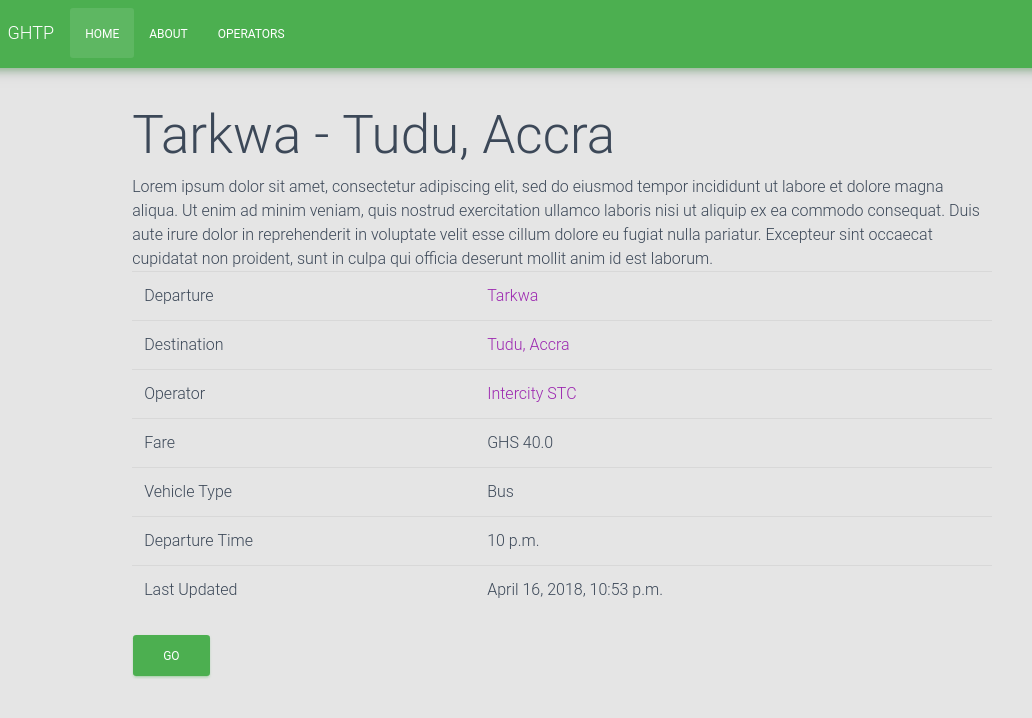
\includegraphics[width=1\linewidth]{routeinfo}
	\caption[Route Information]{Route Information}
	\label{fig:routeinfo}
\end{figure}

-- View Routing on map
View station detail






% ---------------------------------------------------------------------------
%: ----------------------- end of thesis sub-document ------------------------
% ---------------------------------------------------------------------------

